\chapter{Coatings for CAST}
Afte the launch of NuSTAR, the X-ray optics group at DTU Space was invited to participate in the creation of an X-ray optic for the CAST solar axion helioscope. CAST is an experiment at CERN that looks for the hypothetical axion particle which is a solution to the charge-parity (CP) problem of the standard model in particle physics. If the axion exist, it is also some or all of the dark matter in the universe. It was assumed that the technology from NuSTAR could be leveraged and therefore use spare glass to make a cheap and relatively simple X-ray optic.

The optic was designed between summer 2012 and summer 2014. Production, assembly, installation and alignment with CAST was done during summer 2014 in cooperation with University of Zaragoza in Spain and Lawrence Livermore National Lab in the US. In this chapter the reader will find a description of the whole process from start to finish.

\section{The CAST instrument}

The axion is an ultra-light particle that is formed from the interaction of a photon with an electromagnetic field, called the Primakoff effect. So the main sources of the particle would be from inside stars, and from Earth the best nearby source will of course be the Sun. The axion is weakly interacting so in order to detect it, CAST uses a strong magnet to convert the axion back to a photon again by the Primakoff effect. The photons subsequently hit a detector.

\begin{figure}[htbp]
  \centering
    \includegraphics[height=6cm]{figures/cast/axion_spectrum.png}
  \caption{}
  \label{fig:axion_spectrum}
\end{figure}

The spectrum of X-rays from axions can be seen in figure \ref{fig:axion_spectrum}. It is relatively low energy X-rays with a peak around 3 keV and a shape similar to the black-body radiation spectrum.

\begin{figure}[htbp]
  \centering
    \includegraphics[height=6cm]{figures/cast/axion_search_cast.pdf}
  \caption{}
  \label{fig:axion_search_cast}
\end{figure}

From theory, the expected mass of the axion is between $10^{-7}$-$1$ eV. In figure \ref{fig:axion_search_cast} the search area can be seen as the axion-photon coupling constant, \gay, as a function of the axion mass, \maxion. The yellow line represents the area where we expect to see the axion if all dark matter in the universe consists of axion particles with the same \maxion\ and \gay. The CAST helioscope is by 2014 the most comprehensive axion search, and has set an experimental upper limit of
\begin{eqnarray}
\gaymath \leq 2 \cdot 10^{-10} \textrm{ GeV}^{-1}.
\end{eqnarray}
% \begin{figure}
% \centering
% \begin{minipage}{.5\textwidth}
%   \centering
%   \includegraphics[height=4.6cm]{figures/cast/axion_spectrum.png}
%   \captionof{figure}{A figure}
%   \label{fig:axion_spectrum}
% \end{minipage}%
% \begin{minipage}{.5\textwidth}
%   \centering  \includegraphics[width=\linewidth]{figures/cast/axion_search_cast.pdf}
%   \captionof{figure}{Another figure}
%   \label{fig:axion_search_cast}
% \end{minipage}
% \end{figure}
The CAST experiment is largely made from spare parts of other projects at CERN and other research institutions. The magnet is one of three prototype superconducting dipole magnets from the Large Hadron Collider. It is designed to transport particles in two directions inside a strong magnetic field, so it has two bores inside with diameters of 43 mm. As can be seen in the picture of the CAST instrument (figure \ref{fig:cast_instrument}), the magnet is able to pitch and yaw up to a limit. That makes it possible to follow the sun as it comes up with one end and as it goes down with the other end. Since the axion does not interact with matter, detectors are placed at both ends of the magnet and at both boreholes, so two detectors can be used at sunrise and two at sunset.

\begin{figure}[htbp]
  \centering
    \includegraphics[height=5cm]{figures/cast/cast_instrument.jpg}
  \caption{}
  \label{fig:cast_instrument}
\end{figure}

!!!!!!!Something about Micromegas detectors!!!!!

CAST has been doing axion searches since 2002 and the experiment continually improves and reiterates the equipment to get higher sensitivity. One major problem is to get a high enough signal-to-noise ratio, the majority of the noise coming from background radiation from the ground, the materials and also cosmic rays.

The detectors covers the entire area of each bore opening, so are relatively large. Detector size is proportional to the background radiation, so it makes sense to have smaller detectors. By using X-ray optics, the X-ray photons can be focused into a detector area of only a fraction of the previous. This will significantly increase the signal-to-noise ratio and will let the CAST helioscope search for the axion in new areas.

\section{Developing an optic for CAST}
One major concern in making an X-ray optic from NuSTAR glass for the CAST helioscope is the limited space available. The optic would have to fit on the end of the magnet nearest the wall, which leaves only about 2 meters for optic, detector and the focal length between the two. Another problem is the small bore opening of only 43 mm, which is smaller than the inner radius of the NuSTAR telescopes. Both of those problems can be solved by realising that the optic would not require imaging capability and the axion spectrum is of relatively low energies.

!!!Diagram of CAST exp. hall from top, shows the limited space!!!

\begin{figure}[htbp]
  \centering
    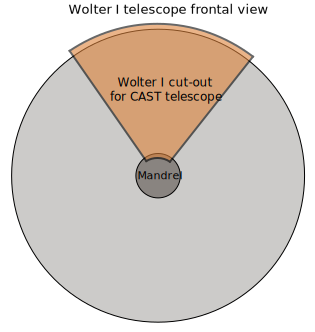
\includegraphics[height=5cm]{figures/cast/wolter1-cutout.pdf}
  \caption{}
  \label{fig:wolter1-cutout}
\end{figure}

By using only 1/6 of the Wolter I radial reflective area, a pie-slice (figure \ref{fig:wolter1-cutout}), two stacks of mirrors can be used to reflect X-rays to one side. The stack only needs to be high enough to cover the bore opening, but each mirror should also be wide enough. The NuSTAR glass pieces are made in 60\degr\ segments for the inner radii and 30\degr\ segments for the outer radii.

\subsection{Optic geometry considerations}
The geometry of the optic was calculated using the following equation for a Wolter I optic:
\begin{eqnarray}\label{eq:wolter}
  \tan(4\alpha) = \frac{\mathit{R3}}{f},
\end{eqnarray}
where $\alpha$ is the angle of reflection of each mirror, $f$, is the focal length and $\mathit{R3}$ is the radius between center of optic and the midpoint between parabolic and hyperbolic mirror (figure \ref{fig:wolter1-diagram}). The center of the bore will need an off-set with the focal plane of the telescope, given by $d$, which is the radius of the bore, $r_{\text{bore}}$, plus the minimum radius of a NuSTAR optic, $r_{\text{min}}$. The length of the NuSTAR mirrors is $l = 225$ mm.
% \begin{figure}
% \centering
% \begin{minipage}{.5\textwidth}
%   \centering
%   \includegraphics[width=\linewidth]{figures/cast/wolter1-diagram.eps}
%   \captionof{figure}{Diagram of wolter I from side.R1-R5 designated.}
%   \label{fig:wolter1-diagram}
% \end{minipage}%
% \begin{minipage}{.5\textwidth}
%   \centering  \includegraphics[width=\linewidth]{figures/cast/axion_search_cast.pdf}
%   \captionof{figure}{Show bore-opening with mandrel from front.}
%   \label{fig:optic_and_bore}
% \end{minipage}
% \end{figure}
\begin{figure}[htbp]
  \centering
    \includegraphics[width=0.95\linewidth]{figures/cast/wolter1-diagram.eps}
  \caption{Diagram of wolter I from side.R1-R5 designated.}
  \label{fig:wolter1-diagram}
\end{figure}

The focal length $f$ was set to a fixed value of 1.5 m. Using $r_{\text{min}}$ as the 0th layer radius, $\mathit{R3}_0$, the angle of the first layer, $\alpha_0$, can be calculated using eq. \ref{eq:wolter}. From $\alpha_0$ and $\mathit{R3}_0$, we can calculate $\mathit{R1}_0$, $\mathit{R2}_0$, $\mathit{R4}_0$ and \ensuremath{\mathit{R5}_0}:
\begin{eqnarray}
  \mathit{R2}_i &=& \mathit{R3}_i + 0.5\ x_{\text{sep}}\tan(\alpha_i),\\
  \mathit{R1}_i &=& \mathit{R2}_i + l\sin(\alpha_i),\\
  \mathit{R4}_i &=& \mathit{R3}_i - 0.5\ x_{\text{sep}}\tan(3\alpha_i),\\
  \mathit{R5}_i &=& \mathit{R4}_i - l\sin(3\alpha_i),
\end{eqnarray}
for layer $i=0$, where $x_{\text{sep}}$ is the distance between the parabolic and hyperbolic mirror. $\mathit{R4}_1$ and $\mathit{R5}_1$ will be a lower value than $r_{\text{min}}$, so it was nessecary to increase the bore to focal plane distance, $d$.

The next layer can be added by setting $\mathit{R3}_{i+1} = \mathit{R1}_i + d_{\text{glass}}$, where $d_{\text{glass}}$ is the thickness of the glass. Thereby the opening of the next layer will be exactly large enough for all incoming photons to hit the parabolic mirror. All mirror layers are subsequently added using the same method until the stack is high enough to cover the bore opening:
\begin{eqnarray}
  \mathit{R1}_{\text{last}} &\geq& r_{\text{min}} + 2r_{\text{bore}}.
\end{eqnarray}

\begin{figure}[htbp]
\centering
\begin{minipage}{.5\textwidth}
  \centering
  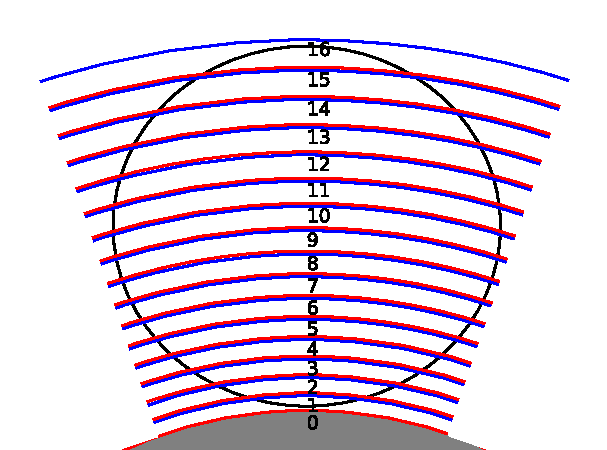
\includegraphics[height=4cm]{figures/cast/cast_front.pdf}
  \captionof{figure}{\footnotesize CAST XRT from front.}
  \label{fig:cast_front}
\end{minipage}%
\begin{minipage}{.5\textwidth}
  \centering  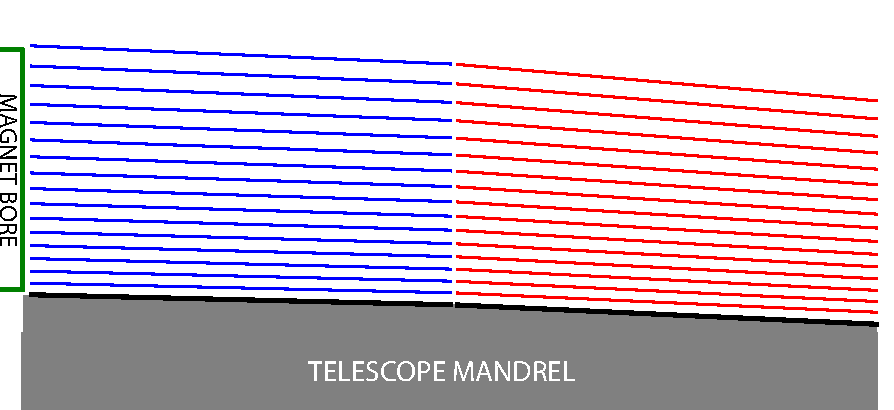
\includegraphics[width=\linewidth]{figures/cast/cast_side.pdf}
  \captionof{figure}{\footnotesize CAST XRT from side.}
  \label{fig:cast_side}
\end{minipage}
\end{figure}

The calculated geometry can be seen in figure \ref{fig:cast_front} and \ref{fig:cast_side}. The calculated radius and angle for each layer can be seen in table \ref{tab:cast_geometry}. The area is the cross sectional area of the layer opening which overlaps with the magnet bore opening, a description of the calculation can be seen in section \ref{sec:eff_area}.

\begin{table}[!h]
\begin{center}
\begin{tabular}{c|c|c|c|c|c}
Layer & Area [mm$^2$] & $\alpha$ [\degr] & $\alpha$ [mrad] & $\mathit{R1}$ [mm] & $\mathit{R5}$ [mm]\\
\hline
0&0.000&0.556&9.697&60.500&51.321 \\
1&13.863&0.579&10.113&63.006&53.821 \\
2&48.175&0.603&10.530&65.606&56.043 \\
3&69.270&0.628&10.962&68.305&58.348 \\
4&86.760&0.654&11.411&71.105&60.741 \\
5&102.266&0.680&11.877&74.011&63.223 \\
6&116.172&0.708&12.360&77.027&65.800 \\
7&128.419&0.737&12.861&80.157&68.474 \\
8&138.664&0.767&13.382&83.405&71.249 \\
9&146.281&0.798&13.921&86.775&74.129 \\
10&150.267&0.830&14.481&90.272&77.117 \\
11&149.002&0.863&15.062&93.902&80.218 \\
12&139.621&0.898&15.665&97.668&83.436 \\
13&115.793&0.933&16.290&101.576&86.776 \\
14&47.648&0.970&16.938&105.632&90.241
\end{tabular}
\end{center}
\caption{\footnotesize Grh gurehiuf wehui fwhguierhui}\label{tab:cast_geometry}
\end{table}

\subsection{Optimising reflective coatings}
To achieve the maximum possible efficiency of the optic, the coating needed to be optimised for the energy range. In contrast with most astrophysical observatories, the CAST telescope will only look at a single object with a very specific spectrum. That means that the coatings can be tailored to achieve maximum reflectivity in that area of the spectrum. Also known is the quantum efficiency of the detector.

An algorithm was developed to calculate all the different permutations of multilayers for a wide variety of material combinations. The spectrum is at a very relatively low X-ray energy, so single layer coatings could be relevant. The algorithm calculates the reflectivity for a multilayer with given material combination and geometry at a certain angle. $F.O.M.$ is then calculated using the following integral:
\begin{equation}\label{eq:fom}
	F.O.M. = \int_{0.1}^{10} R^2(\mathrm{\alpha},\text{E})\ QE_{\text{det}}(\text{E})\ S_{\text{axion}}(\text{E})\ dE,
\end{equation}
with $R^2(\mathrm{\alpha},\text{E})$ being the squared reflectivity because of the double reflection, $QE_{\text{det}}(\text{E})$ the detector quantum efficiency and $S_{\text{axion}}(\text{E})$ the axion spectrum as seen in figure \ref{fig:axion_spectrum}. By integrating over the energy range from 0.1 keV to 10 keV, a figure of merit can be obtained that takes both coating, spectrum and detector into account.

The material combinations considered were multilayers of W/B$_4$C, W/Si, Pt/C, Pt/B$_4$C, Ni/B$_4$C as well as single layers of W, Pt, Ir and Ni. W/Si and Pt/C were the most well understood for slumped glass type substrates, since they both were used in the NuSTAR mission. To find the optimal coating, the parameter space considered for each material combination can be seen in table \ref{tab:cast_parameter_space}. By using $d_{\text{min}}$ and $d_{\text{max}}$, both linearly graded-d coatings and constant-d coatings can be computed. To avoid computing cases where \(d_{\text{min}}\) is larger than \(d_{\text{max}}\), the condition \(d_{\text{min}}\) $\leq$ \(d_{\text{max}}\) has been set.

\begin{table}[!h]
\begin{center}
\begin{tabular}{c|c|c|c}
Parameter & Minimum & Maximum & Interval \\
\hline
$N$ & 1 layer & 30 layers & 1 layer \\
$d_{\text{min}}$ & 3 nm & 300 nm & 0.5 nm \\
$d_{\text{max}}$ & 3 nm & 300 nm & 0.5 nm \\
$\Gamma$ & 0.1 & 0.9 & 0.05 \\
\end{tabular}
\end{center}
\caption{\footnotesize Grh gurehiuf wehui fwhguierhui}\label{tab:cast_parameter_space}
\end{table}

For single layer coatings, only a single thickness of 50 nm was considered. The surface and interface roughnesses were fixed at 0.5 nm. The complete computation was done for every layer in the optic, as $\alpha$ changes throughout the mirror stack. The algorithm does the following steps:
\begin{itemize}
  \item[\bf 1] Finds the next combination in the parameter matrix.
  \item[\bf 2] Calculates the reflectivity using IMD's FRESNEL function.
  \item[\bf 3] Uses the calculated reflectivity in the $F.O.M.$ equation \ref{eq:fom}.
  \item[\bf 4] If the calculated value is higher than the previous maximum value, the parameters are saved and the calculated value set as the new maximum.
\end{itemize}

When the entire parameters space has been covered for a mirror layer and material combination, the algorithm saves the best $F.O.M.$ value and the coating recipe and goes on to the next layer. When all layers are covered, the effective area is calculated and then the algorithm continues on to the next material combination. Calculating the effective area is explained in detail in section \ref{sec:eff_area}. The result of a full computation using the algorithm is shown in figure \ref{fig:mat_result}.

\begin{figure}[htbp]
  \centering
    \includegraphics[height=5cm]{figures/cast/mat_result.png}
  \caption{\footnotesize Effective area comparison for computed material combinations in the CAST XRT optic.}
  \label{fig:mat_result}
\end{figure}

The best result for the W/B$_4$C material combination can be seen in figure \ref{fig:w-b4c-result-1} and \ref{fig:w-b4c-result-2}.

\begin{figure}[htbp]
\centering
\begin{minipage}{.5\textwidth}
  \centering
  \includegraphics[width=\linewidth]{figures/cast/w-b4c-result-1.png}
  \captionof{figure}{\footnotesize }
  \label{fig:w-b4c-result-1}
\end{minipage}%
\begin{minipage}{.5\textwidth}
  \centering  \includegraphics[width=\linewidth]{figures/cast/w-b4c-result-2.png}
  \captionof{figure}{\footnotesize }
  \label{fig:w-b4c-result-2}
\end{minipage}
\end{figure}

The coating optimization for the CAST X-ray optic was done in parallel with most of the ATHENA coating investigations that is described in chapter \ref{chap:athena_coatings}. The findings from long term storage that are discussed in section \ref{sec:long_term} show changes in the coatings over time at ambient conditions for most B$_4$C containing films. For that reason, it was decided to make the CAST coatings with Pt/C, as the combination is well described for NuSTAR like glass substrates. W/Si was also used for NuSTAR and would be a cheaper solution, but the Si absorption line at $\sim2$ keV would decrease efficiency of the coatings around the peak of the axion spectrum.
%Each calculation was done over the energy range $0.1 - 10$ keV with a step size of 0.1 keV.


\subsection{Calculating effective area}\label{sec:eff_area}
The effective area is the cross sectional opening of the optic multiplied with the reflectivity squared for each layer. Total effective area is the sum of effective area of each layer:
\begin{eqnarray}
  A_{\text{eff,i}} &=& A_{\text{CS,i}}R_i^2(\text{E})\\
  A_{\text{eff}} &=& \sum_{i=0}^n A_{\text{eff,i}}
\end{eqnarray}
The cross sectional opening is the intersection of the circle of the bore opening and a layer opening. The layer opening is the cross sectional area between two circles of radius $\mathcal{R}_{i}$ and $\mathcal{R}_{i-1}$, where $\mathcal{R} = \mathit{R1}$. It can be calculated using the overlap of the outer shell of the layer opening and the bore opening. From that is subtracted the overlap of the inner shell of the layer opening with the bore opening as seen in figure \ref{fig:cross_section_area}.

\begin{figure}[htbp]
  \centering
    \includegraphics[width=0.9\linewidth]{figures/cast/cross_section_area.eps}
  \caption{\footnotesize }
  \label{fig:cross_section_area}
\end{figure}

Area of the overlap of $i$th shell with bore is:
\begin{eqnarray}\label{eq:overlap1}
  A_{i} &=& r_{\text{bore}}^2\cos^{-1}\Big(\frac{d^2+r_{\text{bore}}^2-\mathcal{R}_{i}^2}{2dr_{\text{bore}}}\Big)\nonumber\\
  &&+\mathcal{R}_{i}^2\cos^{-1}\Big(\frac{d^2-r_{\text{bore}}^2+\mathcal{R}_{i}^2}{2d\mathcal{R}_{i}^2}\Big)\nonumber\\
  &&-\frac{1}{2}\sqrt{(-d+r_{\text{bore}}+\mathcal{R}_{i})(d+r_{\text{bore}}-\mathcal{R}_{i})}\nonumber\\
  &&\times\sqrt{(d-r_{\text{bore}}+\mathcal{R}_{i})(d+r_{\text{bore}}+\mathcal{R}_{i})},
  %A_{i-1} &=&
\end{eqnarray}
Area of the overlap of shell $i-1$ with bore is:
\begin{eqnarray}\label{eq:overlap2}
  A_{i-1} &=& r_{\text{bore}}^2\cos^{-1}\Big(\frac{d^2+r_{\text{bore}}^2-\mathcal{R}_{\text{bot}}^2}{2dr_{\text{bore}}}\Big)\nonumber\\
  &&+\mathcal{R}_{\text{bot}}^2\cos^{-1}\Big(\frac{d^2-r_{\text{bore}}^2+\mathcal{R}_{\text{bot}}^2}{2d\mathcal{R}_{\text{bot}}^2}\Big)\nonumber\\
  &&-\frac{1}{2}\sqrt{(-d+r_{\text{bore}}+\mathcal{R}_{\text{bot}})(d+r_{\text{bore}}-\mathcal{R}_{\text{bot}})}\nonumber\\
  &&\times\sqrt{(d-r_{\text{bore}}+\mathcal{R}_{\text{bot}})(d+r_{\text{bore}}+\mathcal{R}_{\text{bot}})},
\end{eqnarray}
where
\begin{eqnarray}\label{eq:overlap2}
  \mathcal{R}_{\text{bot}} &=& \mathcal{R}_{i-1} + d_{\text{glass}},
\end{eqnarray}
with $\mathcal{R}_{i-1}$ being the radius of the layer underneath layer $i$ and $d_{\text{glass}}$ being the thickness of the glass.

The NuSTAR type telescope is built up from glass layers with graphite spacers between.  Since the optic is so small, but with relatively large openings between the layers, it is necessary to use graphite spacers in the middle. Each of those are rectangular in shape, as high as the opening and $x_{\text{gr}}=2$ mm wide. The spacer obscures the opening, so will have to be subtracted from cross sectional opening. The cross sectional area of the  opening of layer $i$ is then:
\begin{eqnarray}
  A_{\text{CS,i}} &=& A_{i} - A_{i-1} - (\mathcal{R}_{i}-\mathcal{R}_{i-1})x_{\text{gr}}
\end{eqnarray}
The effective area for the optimized Pt/C coating can be seen in figure \ref{fig:eff_area_ptc}.

!!!!! Show eff area here !!!!!!!!
\section{Producing coated substrates}
jhgir agrsi hgrsl ngjkfsdlnburilsn buires

\subsection{Collecting substrates for coating}

\subsection{Coating of substrates}



\section{Assembling coated substrates}


\subsection{Acquiring parts for assembly vacuum vessel}


\section{Installation of optic at CAST}


\subsection{Optic alignment}

\subsection{Tests with 8 keV X-ray source}

\section{Conclusion}
%\section{First light}
